\documentclass{article}
\usepackage{graphicx} % Required for inserting images
\usepackage{hyperref}
\usepackage{subcaption}
\usepackage{float}

\title{Mechatronics. Numerical Experiments}
\author{Ekaterina Mozhegova}
\date{December 2024}

\begin{document}

\maketitle

\section*{Abstract}

\textbf{The second part of the actuator sizing task: choosing custom motors for the UR3 manipulator.}

The first part can be accessed in this \href{https://github.com/illusoryTwin/ActuatorSizing/tree/main}{repository}.

\subsection*{Project Structure}

The Numerical Experiments task can be accessed in my \href{https://github.com/illusoryTwin/NumericalExperimentsforActuatorSizing}{GitHub repository}.

\begin{itemize}
    \item In the `model` folder, you can find all 4 XML models with different motors created for the previous task.  
    \item In the `src` folder, you can see the source code for the conducted experiments.
    \item In the `data` folder, you can find the results of the experiments - torque values for each of the 4 models.
    \item In the `plots` folder, you can see the plots of torques as a result of the experiments.
\end{itemize}


\section{Motor Selection Algorithm}

For the motor selection algorithm, we need to consider the following main aspects:

\begin{enumerate}
    \item Geometrical sizes
    \item Inertia ratio, gear ratio
    \item Torques (maximum allowed torques)
\end{enumerate}

I focused exactly on these criteria while choosing the motors for the UR3 manipulator


\subsection{Sizes}

Firstly, I checked the sizes of the motors and compared them with the sizes of the manipulator.


\begin{figure}[H]
\centering
\begin{subfigure}{0.45\textwidth}
    \centering
    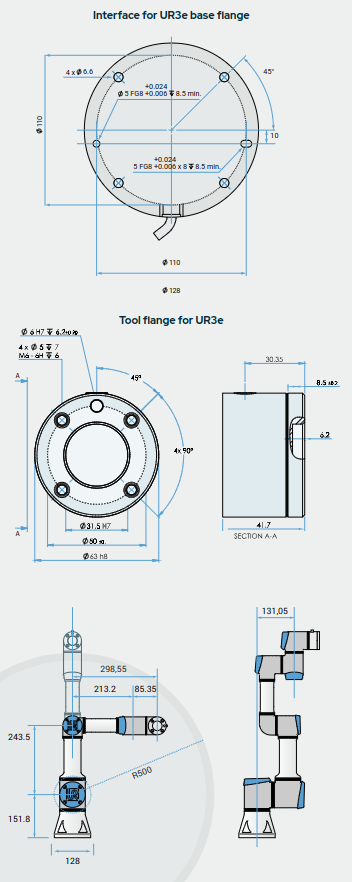
\includegraphics[scale=0.35]{manipulator_sizes.png}
    \caption{Manipulator Sizes}
\end{subfigure} 
\hfill
\begin{subfigure}{0.45\textwidth}
    \centering
    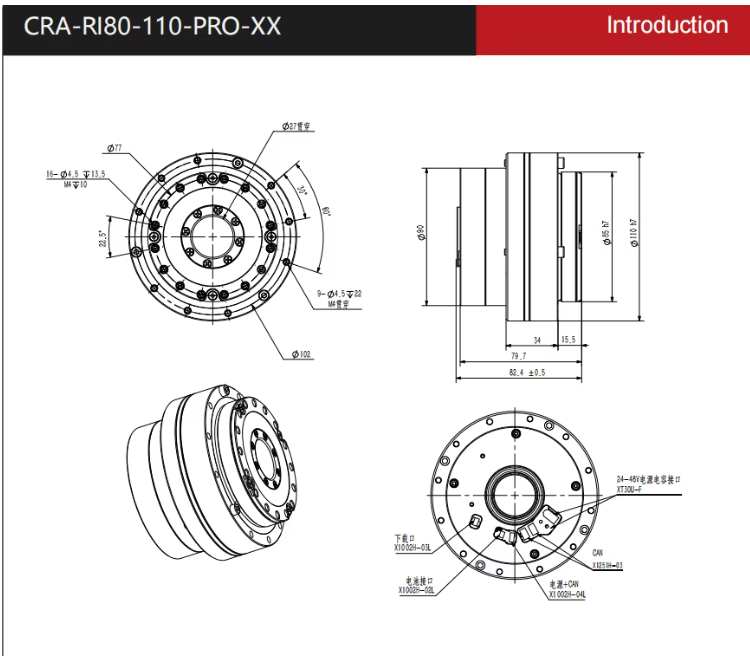
\includegraphics[scale=0.25]{motor_sizes.png}
    \caption{Motor Sizes}
\end{subfigure}
\end{figure}


These comparisons led me to the following options for motors:

\begin{enumerate}
    \item \textbf{CRA-RI80-110-PRO-XX}
    \item \textbf{CRA-RI80-110-NH-XX}
\end{enumerate}

\subsection{Gear Ratios}

I chose the gear ratios with the following reasoning in mind:  

Shoulder joints require more powerful motors, which means higher gear ratios. In contrast, the wrist joint requires the lowest gear ratio since it needs to rotate with a relatively high speed.  

Therefore, for the shoulder joints, I used large gear ratios, 161:1 or 121:1.  
For the elbow joint, I used a smaller ratio of 121:1 or 101:1.  

The smallest gear ratio was used for the wrist joint, with a ratio of 51:1.

\subsection{Configuration Combinations}

Based on criteria 1 and 2, I created four configuration combinations for the manipulator.

You can find them in this \href{https://github.com/illusoryTwin/ActuatorSizing/tree/main}{repository}.

\subsection{Experimental Results}

I conducted both static and dynamic experiments to calculate the torque values on the motors in both static and dynamic conditions.  


Next, I compared the obtained values with the maximum allowable torque from the motor's reference to ensure the motor does not exceed these limits.  

For all 4 generated models, there were some problems with the 1st motor (for the 1st joint) in both static and dynamic experiments and some problems with the 3d motor (for the 3d joint correspondingly) in dynamic experiments: 
the obtained results appeared to be extremely high. 

Probably, the problem was exactly with the way I conducted experiments and not with the motors themselves.

In other cases, the torque values for other motors lied within the acceptable range, so they datisfy the requirements.  

Thus, I can conclude that the following motors are well-suited for the following joints:

\begin{itemize}
    \item wrist joints: 

        - \textbf{CRA-RI80-110-PRO-XX} (gear ratio 51:1)
        
        - \textbf{CRA-RI80-110-NH-XX} (gear ratio 51:1)

    \item shoulder lift joint:
    
        - \textbf{CRA-RI80-110-NH-XX} (101:1)
        
        - \textbf{CRA-RI80-110-PRO-XX} (101:1)
    
\end{itemize}

\end{document}